\documentclass[a4paper,12pt]{article}
\usepackage[utf8]{inputenc}
\usepackage[frenchb]{babel}
\usepackage{setspace}
\usepackage[pdftex]{graphicx}
\usepackage{amsmath}
\usepackage{amssymb}
\usepackage{xcolor}
\usepackage{natbib}
\usepackage{hevea}
\usepackage{footnote}
\usepackage{geometry}
\usepackage{enumitem}
\setlist[enumerate]{leftmargin=*,labelindent=3mm}
\setlist[itemize]{leftmargin=*,labelindent=3mm}
\graphicspath{{img/}}
\geometry{top=2.5cm,bottom=2cm,left=2cm,right=2cm}
\begin{document}
%TEXFILE_JBM_BEGIN

\title{\textbf{TP d'introduction}\\
Utilisation du modèle \texttt{eduplanet}}
\author{\normalsize{Jean-Baptiste Madeleine, Aymeric Spiga}}
\date{Lundi 20 février 2017}

\maketitle

\renewcommand{\labelitemi}{\textbullet}

\section{Introduction}


\subsection{Le modèle climatique utilisé}

\texttt{eduplanet} est une surcouche d'un Modèle de Climat Global complet (aussi appelé
Global Climate Model ou GCM). Il est basé sur une version générique
(c'est-à-dire adaptée à tout type de planète) du modèle \texttt{LMDz}\footnote
{Du nom du laboratoire associé, le Laboratoire de Météorologie Dynamique;}. Ce
modèle, développé sur le campus de l'UPMC, est utilisé pour les simulations de
changement climatique terrestre du GIEC\footnote{Groupe d'experts
Intergouvernemental sur l'\'Evolution du Climat;}, ainsi que pour la simulation
de nombreuses planètes du système solaire (Mars, Vénus, Saturne\dots) et
exoplanètes. Afin de faire des expériences sur des temps de calculs courts,
nous utiliserons dans un premier temps le modèle \texttt{eduplanet} avec peu de
points en espace (8~points selon la longitude~$x$, 8~points selon la
latitude~$y$ et 16~points selon l'altitude~$z$, ce qui correspond environ à des
mailles de 5000~km sur 2500~km). De plus, nous désactivons pour commencer le
c\oe ur dynamique (ou noyau dynamique) du modèle, qui permet de simuler les
vents, afin de nous concentrer sur le rayonnement et l'énergie solaire. Nous
activerons ensuite le c\oe ur dynamique du modèle en fin de TP afin d'étudier
les vents, source de l'énergie éolienne.

\subsection{Méthodes}

\begin{itemize}
\item Le modèle climatique utilisé fonctionne sur Linux. Nous utiliserons par
conséquent une console Linux avec laquelle vous vous familiariserez
progressivement en utilisant la Fiche Pratique n$^\circ$1.
\item Analyser les résultats de vos expériences numériques nécessite de bien
comprendre les différentes variables climatiques et leur signification
physique. Celles-ci sont résumées dans la Fiche Pratique n$^\circ$2.
\item Enfin, l'ensemble de vos expériences doivent être rigoureusement notées,
par exemple dans un fichier texte, avec le nom du dossier de l'expérience et
les principaux réglages. Autrement, vous oublierez rapidement à quoi
correspondent les différents dossiers.
\end{itemize}

\section{Installation du modèle climatique}

Cette première partie du TP consiste à installer le modèle climatique \texttt
{eduplanet} et le logiciel de visualisation des résultats \texttt
{planetoplot}\footnote{Pour plus d'informations, voir
\texttt{https://github.com/aymeric-spiga/planetoplot}}. Les installations
prennent parfois plusieurs minutes. Pendant ces moments d'installation, vous
pouvez lire la suite du TP ainsi que les Fiches Pratiques.

Commencer par ouvrir un terminal de commande Linux. Pour cela, une fois le
bureau Mandriva\footnote{La version de Linux que nous utilisons;} ouvert,
cliquer sur le menu Démarrer (étoile en bas à gauche de l'écran) puis sur
``Outils $>$ Konsole''.

\begin{enumerate}
\item Ouvrir un terminal et créer un dossier nommé WORK à l'emplacement de
votre choix (commande \texttt{mkdir WORK}, voir Fiche n$^\circ$1);
\item Se rendre dans le dossier WORK nouvellement créé à l'aide de la commande
\texttt{cd WORK};
\item Une fois dans le dossier WORK, y installer le modèle \texttt{eduplanet}
en tapant les commandes suivantes (appuyer sur la touche Entrée entre chaque
ligne de commande pour l'exécuter):

\begin{verbatim}
git clone https://github.com/aymeric-spiga/eduplanet eduplanet
cd eduplanet
./fix/upmc_set.sh
\end{verbatim}

Taper ensuite \texttt{source $\sim$/.bashrc} comme indiqué par le programme,
puis poursuivre en tapant:

\begin{verbatim}
./install.sh
\end{verbatim}

L'installation dure environ 20~minutes. Elle n'est à faire qu'\textbf{une seule
fois}.

\item Une fois l'installation terminée, lancer une première expérience en
tapant simplement:

\begin{verbatim}
./run.sh
\end{verbatim}

Des lignes défilent en affichant la longitude solaire \texttt{Ls}. La longitude
solaire indique la position de la Terre autour du Soleil
(voir Figure~\ref{fig-solarlon}). C'est notre repère temporel. Un axe en $L_s$
(en degrés) donnera donc l'évolution temporelle des variables du modèle.
Attendre la fin de l'expérience.

\begin{figure}[htbp]
\centering
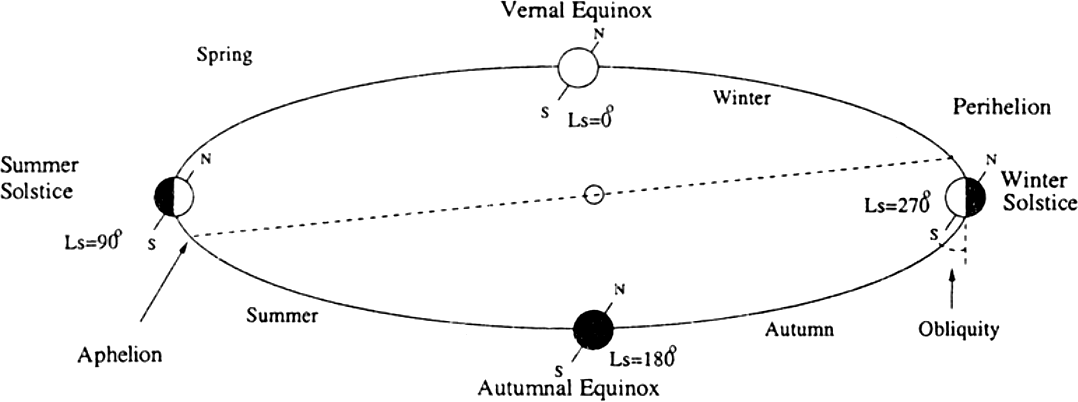
\includegraphics[width=14cm]{fig-3T054-Ls.png}
\caption{Longitude solaire $L_s$ de la Terre autour du Soleil. Le solstice
d'été dans l'hémisphère Nord est à $L_s=90^\circ$, et le solstice d'hiver à
$L_s=270^\circ$. La longitude solaire à laquelle la planète est au plus proche
du Soleil (périhélie) est souvent notée $L_p$ (ici $L_p \simeq 280^\circ$).}
\label{fig-solarlon}
\end{figure}

\item Un fois l'expérience terminée, vérifier avec la commande \texttt{ls}
qu'un dossier nommé \texttt{expnum\-\_DATE\--ET\--HEURE} a bien été créé. Ce
dossier contient les résultats de l'expérience (fichier \texttt{resultat.nc})
ainsi qu'une sauvegarde des réglages utilisés pour l'expérience (fichiers
\texttt{regla\-ges\_\-init.txt} et \texttt{reglages\_\-run.txt}).
\end{enumerate}




\section{Analyse de la première expérience}
\label{sct-analyse}

\subsection{Réglages de l'expérience}

Avant d'analyser les résultats de l'expérience réalisée ci-dessus, nous
documentons les réglages associés. Ces réglages sont renseignés dans les
fichiers \texttt{reglages\_init.txt} et \texttt{reglages\_run.txt}.

\begin{enumerate}
\item Ouvrir avec un éditeur de texte le fichier \texttt{reglages\_init.txt}
tout en veillant à ne pas le modifier. Les lignes correspondant à des
paramètres de l'expérience sont indiquées par des flèches. Noter et définir ces
différents paramètres.
\item L'inertie thermique de la surface dans cette expérience est-elle
relativement élevée ou faible?

On rappelle quelques valeurs typiques de l'inertie thermique:

\begin{table}[h!]
\centering
\begin{tabular}{c|c|c|c}
& Désert & Roches & Océan \\ \hline
Inertie thermique (en tiu = J~K$^{-1}$~m$^{-2}$~s$^{-1/2}$): & 50 tiu &
400 tiu & 18000 tiu \\
\end{tabular}
\end{table}
\end{enumerate}

\subsection{Affichage des résultats}
\label{sct-display}

La commande \texttt{atlas.py} contenue dans le dossier \texttt{TOOLS} permet de
tracer les résultats d'une expérience en affichant successivement les
principales variables climatiques (voir la Fiche Pratique n$^\circ$2). Afin de
visualiser les résultats de la première expérience, lancer la commande \texttt
{./TOOLS/atlas.py} suivi du nom de fichier de résultat de la première
expérience\footnote{Pour compléter automatiquement le chemin vers ce fichier,
utiliser la touche \texttt{TAB};}:

\begin{verbatim}
./TOOLS/atlas.py expnum_DATE-ET-HEURE/resultat.nc
\end{verbatim}

Une série de figures s'affiche (fermer chaque fenêtre pour passer à la
suivante\footnote{Avant de fermer la fenêtre, il est possible de sauvegarder
chaque figure dans le dossier
\texttt{expnum\-\_DATE\--ET\--HEURE} en cliquant sur la disquette en haut à
gauche de la figure.}):
\begin{itemize}
\item \textbf{Figure~1:} La température de surface $T_s$ en fonction de $L_s$
pour différentes latitudes;
\item \textbf{Figure~2:} La température de surface $T_s$ moyenne de l'ensemble
du globe en fonction de $L_s$;
\item \textbf{Figure~3:} Quatres panneaux donnant en fonction du temps et de la
latitude 1) le flux solaire incident au sommet $F_{vis}^{\downarrow_{TOA}}$, 2)
le flux solaire absorbé par la surface $F_{vis}^{\downarrow_{Surf}}$, 3) $F_
{IR}^{\uparrow_{TOA}}$ le flux infrarouge émis au sommet, et 4) la température
de surface $T_s$;
\item \textbf{Figure~4:} La température de l'atmosphère $T$ en fonction de la
pression $p$ (en~Pa) et de la latitude, et ce pour $L_s=90^\circ$ (gauche) et
$L_s=270^\circ$ (droite).
\end{itemize}

\subsection{Cycle saisonnier de la température}

\begin{enumerate}
\item Repérer les saisons sur la Figure~1 et observer les décalages de $T_s$
selon la latitude.
\item Pourquoi $T_s$ à 20$^\circ$S peut-elle être supérieure à $T_s$ à
l'équateur? Quel paramètre vous permet de vérifier cela? \`A quelle $L_s$ et
quelle saison ceci se produit-il?
\end{enumerate}

\subsection{Convergence de l'expérience vers un état d'équilibre}
\label{ssct-equilibre}

\begin{enumerate}
\item Sur la Figure~2, repérer la durée de la réponse transitoire du modèle (en
degrés de $L_s$). C'est la durée nécessaire aux variables du modèle pour
atteindre une répétitivité temporelle et une stabilité statistique. \`A la fin
de cette durée, le modèle atteint l'\textbf{équilibre climatique}. \`A combien
de jours cela correspond dans cette configuration (approximativement) ?
\item Quelle est la température de surface une fois l'équilibre climatique
atteint?
\end{enumerate}

\subsection{Bilan énergétique}

Sur la Figure~3:

\begin{enumerate}
\item Autour de quelle valeur moyenne varie approximativement le flux solaire
incident au sommet $F_{vis}^{\downarrow_{TOA}}$ ? \footnote{Voir la Fiche
Pratique~n$^\circ$2 pour la liste des variables; ``TOA'' signifie ``Top Of
Atmosphere'';}
\item Dans quelles régions du globe les valeurs du flux solaire incident au
sommet $F_{vis}^{\downarrow_{TOA}}$ sont-elles les plus grandes ? Serait-il
intéressant d'y installer des panneaux solaires ?
\item Quelles sont les valeurs maximales de $F_{vis}^{\downarrow_{TOA}}$ et du
flux solaire absorbé par la surface $F_{vis}^{\downarrow_{Surf}}$ (regarder le
maximum de l'échelle de couleur) ? Que vaut le rapport de ces deux valeurs? \`A
quel paramètre théorique peut-on relier cette valeur?
\item Le flux infrarouge sortant au sommet $F_{IR}^{\uparrow_{TOA}}$
reflète-t-il les variations de $F_{vis}^{\downarrow_{Surf}}$ (en haut à droite)
ou bien de $T_s$ (en bas à droite)? Pourquoi le flux infrarouge sortant au
sommet $F_{IR}^{\uparrow_{TOA}}$ ainsi que la température de surface $T_s$ ne
présentent pas exactement les mêmes variations que la densité de flux solaire
absorbée à la surface $F_{vis}^{\downarrow_{Surf}}$ ?
\item En utilisant l'éclairement moyen au sommet de l'atmosphère $E'=342$~W~m$^
{-2}$ (qui doit avoisiner la valeur trouvée à la question 1. ci-dessus) et une
opacité infrarouge $\tau_s = 0.8$, calculer la température théorique de la
surface $T_s$ à l'équilibre radiatif\footnote{On rappelle la constante de
Stefan-Boltzman $\sigma = 5,67\times 10^{-8}$~J~s$^{-1}$~m$^{-2}$~K$^{-4}$;}:

\begin{equation}
T_s = \sqrt[4]{\frac{E'(1-A_b)(1+\frac{\tau_s}{2})}{\epsilon_s \sigma}}
\end{equation}

Ceci est-il en accord avec la température à l'équilibre climatique trouvée dans
la
partie~\ref{ssct-equilibre} ?
\end{enumerate}

\section{Approfondissement des grandeurs liées au rayonnement solaire}

L'orbite de la Terre est définie par ses paramètres orbitaux:

\begin{itemize}
\item Obliquité $\omega$ (actuellement $\omega$~=~23.9$^\circ$): angle entre
l'axe de rotation de la planète et la normale au plan orbital (paramètre
\texttt{obliquit} du modèle);
\item Excentricité $e$ (actuellement $e$~=~0.0167): écart à un cercle, avec
$e=c/a$ (voir Figure~\ref{fig-orbite});
\item Longitude solaire du périhélie $L_p$ (actuellement $L_p$~=~283$^\circ$).
\end{itemize}

\begin{figure}[htbp]
\centering
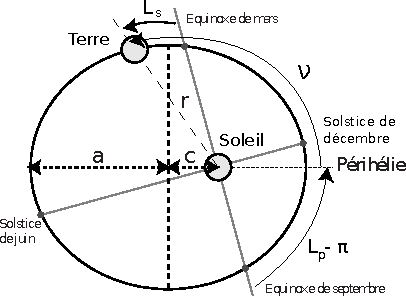
\includegraphics[width=10cm]{fig-3T054-excentricite-nu.pdf}
\caption{Paramètres orbitaux d'une planète. $r$: distance entre la planète et
l'étoile pour la position considérée. $L_s$: longitude solaire de la planète
autour de son étoile à l'instant considéré (angle compté depuis l'équinoxe de
printemps Nord, avec solstice d'été Nord pour $L_s=90^\circ$ et solstice
d'hiver Nord pour $L_s=270^\circ$). $L_p$: longitude solaire du périhélie
(planète au plus proche de son étoile, ici $L_p \simeq 260^\circ$). $\nu$:
anomalie vraie, angle entre la position de la planète au périhélie et la
position considérée ($\nu$ et $L_s$ sont reliés par la relation $\nu = L_s -
L_p$). $e$: excentricité de l'orbite définie par le rapport entre la distance
du foyer au centre de l'ellipse $c$ et le demi grand axe $a$: $e=c/a$ avec $0
\leq e < 1$.}
\label{fig-orbite}
\end{figure}

\begin{enumerate}
\item Reprendre la première expérience de la partie~\ref{sct-analyse}. Sachant
que l'excentricité s'exprime $e=c/a$ et que dans le fichier de réglage \texttt
{reglages\_init.txt}, \texttt{apoastr} = $a+c$ et \texttt{periastr} = $a-c$,
montrer que \texttt{apoastr} = $a(1+e)$ et \texttt{periastr} = $a(1-e)$. Que
vaut $e$ dans cet expérience ?

\item Afficher de nouveau la Figure~3 de l'expérience. La Figure~3 montre en
haut à gauche le flux solaire incident au sommet $F_{vis}^{\downarrow_{TOA}}$.
Ce flux correspond au flux solaire moyen journalier, noté $\bar{I}$ et aussi
appelé insolation moyenne journalière (en W~m$^{-2}$).

\begin{enumerate}
\item Il est possible de démontrer qu'au \textbf{solstice d'été} et au \textbf
{pôle}, la durée du jour est de 24h et $\bar{I}$ s'écrit:
\begin{equation}
\bar{I} = E^\ast \ \sin \omega \text{ , avec } \omega \text{ l'obliquité, et }
E^\ast = E \left(\frac{1+e \cos \nu}{1-e^2} \right)^2.
\end{equation}

En utilisant le résultat précédent, la valeur de la constante solaire $E$
donnée par le paramètre \texttt{Fat1AU} du fichier \texttt{reglages\_run.txt}
et l'obliquité \texttt{obliquit} du fichier \texttt{reglages\_init.txt},
calculer la valeur de $\bar{I}$ attendue au pôle pour le solstice. Est-ce en
accord avec le résultat du modèle?

\item De la même façon, on peut exprimer $\bar{I}$ \textbf{à l'équinoxe} par la
relation:

\begin{equation}
\bar{I}=\frac{E^\ast}{\pi} \ \cos \phi \text{ , avec } \phi \text{ la
latitude.}
\label{eqn-equi}
\end{equation}

Cette dernière expression de $\bar{I}$ correspond à une coupe selon l'axe $y$
et à $L_s$ = 0$^\circ$ ou~180$^\circ$ (les deux équinoxes) de la Figure~3.
Fermer la Figure~3 et retourner dans la console pour tracer $\bar{I}$ à
l'équinoxe d'automne, soit pour $L_s = 180^\circ$. Pour cela, on utilisera la
commande\footnote{On utilise ici le programme \texttt{planetoplot} de façon
interactive, l'option \texttt{-v} désignant la variable, \texttt{-x} la
longitude et \texttt{-t} le temps (dans ce cas la longitude solaire $L_s$).
Pour plus d'information et exemples, voir le wiki \texttt{eduplanet} à cette
adresse : \texttt{https://github.com/aymeric-spiga/eduplanet/wiki};}:

\begin{verbatim}
pp.py expnum_DATE-ET-HEURE/resultat.nc -v ISR -x 0 -t 1799,1801
\end{verbatim}

Quelle fonction trigonométrique reconnaît-on alors? Que vaut le maximum du flux
moyen journalier $\bar{I}$ à $\phi$~=~0? Le vérifier par le calcul\footnote
{Pour des raisons de résolution temporelle des résultats, nous remarquerons que
le flux au pôle ne s'annule pas sur cette courbe. Il s'annulerait bel et bien
si nous avions une sortie du modèle pour un $L_s$ très exactement égal à
180$^\circ$;}.
\end{enumerate}

\end{enumerate}

\section{Ajout des continents}
\label{sct-continents}

Installer la version du code incluant les continents grâce à la commande:

\begin{verbatim}
./updatecode.sh
\end{verbatim}

Ouvrir le fichier de réglage \texttt{reglages\_init.txt} dans un éditeur (par
exemple \texttt{gedit}), puis ouvrir également dans l'éditeur le fichier
\texttt{INIT/planet\_start.earth.continents}.
Copier l'intégralité du contenu du fichier
\texttt{INIT/planet\_start.earth.continents} dans le fichier \texttt
{reglages\_init.txt} en remplaçant l'in\-tégralité des anciens paramètres.
Relancer une expérience avec ces nouveaux réglages grâce à la commande \texttt
{./run.sh}.

\begin{enumerate}
\item Visualiser le nouvel albédo grâce à la commande:
\begin{verbatim}
pp.py -v albedo RUN/DATAGENERIC/surface_earth.nc
\end{verbatim}
Comparer la carte obtenue aux valeurs du tableau~\ref{tab-albedo} et identifier
les principales régions climatiques du globe.
\begin{table}[h!]
\centering
\begin{tabular}{cc}
\textbf{Surface} & \textbf{Albedo} \\ \hline
Bare soil & 0.17 \\
Conifer forest & 0.08 \\
Deciduous forest & 0.15--0.2 \\
Desert sand & 0.40 \\
Fresh snow & 0.80--0.90 \\
Glacier & 0.2--0.4 \\
Green grass & 0.25 \\
Ocean ice & 0.5--0.7 \\
Thick clouds & 0.6--0.9 \\
Water (small zenith angle) & 0.03--0.1 \\
\end{tabular}
\caption{Exemples d'albédo de différents types de surfaces.}
\label{tab-albedo}
\end{table}

\item De même, visualiser l'inertie thermique de la surface grâce à la commande
\begin{verbatim}
pp.py -v thermal RUN/DATAGENERIC/surface_earth.nc
\end{verbatim}
\item Lancer de nouveau l'atlas grâce à la commande \texttt{./TOOLS/atlas.py}.
Sur la Figure~3 montrant quatre panneaux (flux solaire incident au sommet $F_
{vis}^{\downarrow_{TOA}}$, flux solaire absorbé par la surface $F_{vis}^
{\downarrow_{Surf}}$, flux infrarouge émis au sommet $F_{IR}^{\uparrow_{TOA}}$
et température de surface $T_s$), identifier les principaux changements par
rapport aux simulations avec albédo et inertie thermique constantes.
\item Comparer la température de surface $T_s$ à 20$^\circ$N pour 0$^\circ$ de
longitude (Sahara) puis 45$^\circ$W (océan Atlantique) grâce à la commande (sur
une ligne):

\begin{verbatim}
pp.py expnum_DATE-ET-HEURE/resultat.nc -v tsurf
-y 20 -x 0 -x -45 -S -s correctls
\end{verbatim}


\end{enumerate}

\section{Activation du c\oe ur dynamique et calcul des vents}

Afin de lancer séparément les expériences incluant la dynamique, nous
installons de nouveau le modèle. Retourner donc dans le dossier \texttt{WORK}
puis installer de nouveau le modèle:

\begin{verbatim}
git clone https://github.com/aymeric-spiga/eduplanet eduplanet-dyn
cd eduplanet-dyn/
./install.sh
./updatecode.sh
\end{verbatim}

Effectuer ensuite les réglages pour ajouter les continents et la dynamique
(voir partie~\ref{sct-continents}):

\begin{verbatim}
gedit INIT/planet_start.earth.continents &
gedit reglages_init.txt
\end{verbatim}

\`A présent, ouvrir le fichier de réglage \texttt{reglages\_run.txt} et
décommenter (en enlevant un signe \# en début de ligne) le passage suivant:

\begin{verbatim}
#####################
##### DYNAMIQUE #####
#####################

nday = 500
ecritphy = 144
day_step = 240
diurnal = .true.
# periode de la physique (en pas)
iphysiq = 5
# periode pour le pas Matsuno (en pas)
iperiod = 5
\end{verbatim}

Relancer une expérience en utilisant cette fois la commande\footnote{Cette
commande permet de lancer une expérience avec 16 points en longitude et en
latitude, et avec le c\oe ur dynamique (option \texttt{--dyn}).}:

\begin{verbatim}
./run.sh -x 16 -y 16 -z 16 --dyn
\end{verbatim}

Laisser cette fenêtre ouverte. \textbf{Le temps de calcul de cette expérience
est d'environ une demi-heure}. Faire pendant ce temps le début du sujet dans
l'autre dossier \texttt{eduplanet}.

Une fois l'expérience terminée, lancer la même simulation mais sans le c\oe ur
dynamique, pour comparaison\footnote{Remarque: il peut être utile à ce stade de
renommer vos dossiers d'expérience \texttt{expnum} afin de ne pas se perdre
dans vos expériences !}:

\begin{verbatim}
./run.sh -x 16 -y 16 -z 16
\end{verbatim}

\begin{enumerate}
\item Ouvrir l'atlas avec la commande habituelle. Sur la Figure~1, quels
changements observe-t-on lorsque la dynamique atmosphérique est activée ?
\item Sur la Figure~2, comparer la mise à l'équilibre du modèle avec et sans la
dynamique.
\item Quels changements sont constatés sur la Figure~3 et la Figure~4 ?

\item Tracer une coupe du vent zonal $u$ grâce à la commande:

\begin{verbatim}
pp.py expnum_DATE-ET-HEURE/resultat.nc -v u -v temp -t 540 -x 0 -s correctls
\end{verbatim}

\begin{enumerate}
\item Commenter la structure en température ainsi que le vent zonal $u$. Quelle
équation relie ces deux variables ?
\item \`A quelle pression se trouve le maximum de vent zonal $u$ ? \`A quelle
altitude cela correspond-t-il ?
\end{enumerate}

\item Représenter pour $L_s$~=~180$^\circ$ les vents proche de la surface ainsi
que la température grâce à la commande (toujours sur une seule ligne):

\begin{verbatim}
pp.py expnum_DATE-ET-HEURE/resultat.nc -v temp -z 1013e2
-t 540 -i u -j v -B coast -P cyl -W 2 -s correctls
\end{verbatim}

\begin{enumerate}
\item \`A quelle saison correspond cette circulation ?
\item Identifier les grands traits de la circulation atmosphérique.
\item Où sont situés les vents les plus forts ?
\end{enumerate}

\end{enumerate}

\section*{Annexe: Les équations d'un GCM}
%-------------------------------------------------------------------

Le tableau ci-dessous compare les caractéristiques du modèle de bilan
énergétique (MB\'E) simple que l'on peut développer analytiquement (à gauche)
et celles d'un GCM complet (à droite), dont les équations se résolvent par
ordinateur.

\begin{savenotes}
\begin{table}[h!]
\centering
\begin{tabular}{l|l}
\textbf{MB\'E} & \textbf{GCM} \\ \hline
Une variable indépendante: $t$ & 4 variables indépendantes: $x,y,z,t$ \\
Une seule inconnue: $\delta T(t)$ & 6 inconnues\footnote{Toutes dépendantes
de (x,y,z,t).}: $T,\vec{v}(u,v,w),p,\rho$ \\
Une équation pour une inconnue: C\'E & 6 équations: CM, C\'E, CQM
(3$\times$), GP \\
Une ODE avec une CI & Plusieurs PDE avec des CI et CL \\
Une condition initiale $\delta T_0$ & Conditions initiales 3D et limites
(surface+sommet) \\
\end{tabular}
\end{table}
\end{savenotes}

Les six équations d'un GCM sont les suivantes:

\begin{align}
\text{CQM~:~} & \frac{d\underline{v}}{dt} = -2\underline
{\Omega}\times\underline{v} - \frac{1}{\rho}\underline{\nabla} p + \underline
{g} + \underline{F_r} \ \text{(compte triple, trois composantes)} \\
\text{C\'E~:~} & C_p \frac{dT}{dt} = Q + \frac{1}{\rho}\frac{dp}{dt} \
\text{(avec $Q$ les sources/puits d'énergie)} \\
\text{CM~:~} & \frac{1}{\rho}\frac{d\rho}{dt} = -\underline
{\nabla}.\underline{v} \ \text{(l'augmentation de densité correspond à une
convergence)} \\
\text{GP~:~} & p = \rho R T
\end{align}

Ces équations sont des équations aux dérivées partielles (PDE pour partial
differential equations) car les dérivées sont lagrangiennes:

\begin{equation}
\frac{d .}{dt} = \frac{\partial . }{\partial t} + (\underline{v}.\underline
{\nabla}) .
\end{equation}

Ces équations sont appelées équations primitives de la Météorologie.

Le modèle peut aussi transporter des constituants (par exemple des gaz, de la
vapeur d'eau, des nuages) par l'ajout d'une équation d'advection.

Ces équations sont résolues dans le modèle en ajoutant à chaque pas de temps
les \emph{tendances} correspondantes aux différentes processus de façon
explicite. Soit $X(x,y,z,t)$ une des 6 inconnues du modèle :

\begin{align}
X_{t+\Delta t} = X_t & + \left( \frac{\partial X}{\partial t} \right)_
{\text{dyn}} \Delta t \ \text{(c\oe ur dynamique: résout CQM, CM, C\'E)} \\
& + \left( \frac{\partial X}{\partial t} \right)_{\text{ray}} \Delta t \
\text{(transfert radiatif: résout C\'E pour le rayonnement)} \\
& + \left( \frac{\partial X}{\partial t} \right)_{\text{param}} \Delta t \
\text{(paramétrisations physiques)}
\end{align}

De nombreux processus se produisent à une échelle spatiale plus petite que
celle du modèle (la turbulence, les nuages, la neige\dots). \`A l'intérieur
d'une maille du modèle, par exemple pour une maille grossière de 1000~km sur
1000~km centrée sur la France, on ne peut donc pas calculer si il y aura
davantage de nuages à Bordeaux qu'à Paris. On travaille alors sur la
probabilité de trouver un nuage dans cette maille grâce à des équations
physiques et statistiques, dîtes paramétrisations physiques.

Il est possible de réaliser des simulations sans utiliser le c\oe ur dynamique
et sans calculer le terme $(\partial X / \partial t)_\text{dyn}$. Dans ce cas,
seul le transfert de rayonnement a lieu dans l'atmosphère, mais elle n'est pas
mise en mouvement. Il n'y a alors pas de vent.

\medskip

Une simulation GCM sera caractérisée par:

\begin{itemize}
\item Son pas de temps $\Delta t$ (typiquement de l'ordre de plusieurs dizaines
de minutes)
\item Sa résolution spatiale horizontale $\Delta x$, $\Delta y$ et verticale
$\Delta z$ (typiquement plusieurs centaines de km sur l'horizontale et
plusieurs centaines de mètres sur la verticale)
\item Ses conditions initiales ($T_i,p_i,\rho_i,\vec{v}_i$)
\item Ses conditions limites en haut (par exemple la densité de flux solaire
$E$) et en bas (par exemple la topographie)
\item Ses paramètres, c'est-à-dire les grandeurs physiques que l'on choisit
pour le calcul du rayonnement et des paramétrisations physiques, par exemple:
\begin{itemize}
\item $A_b$ l'albédo de la surface
\item $I=\sqrt{\lambda \rho_s C}$ l'inertie thermique
\item $\kappa_\text{IR}$ le coefficient d'absorption IR
\item etc\dots
\end{itemize}
\end{itemize}

En Climatologie, on impose souvent au modèle des conditions limites ou
paramètres variants sur de longues échelles de temps (plusieurs décennies): on
parle alors de forçage climatique. Il ne faut pas confondre forçage et
perturbation, qui a lieu sur le court-terme (par exemple une éruption
volcanique).




%TEXFILE_JBM_END
\end{document}
